\documentclass[11pt,a4paper]{article}

\usepackage[T1]{fontenc}
\usepackage{lmodern}
\usepackage{microtype}
\usepackage{amsmath,amssymb,amsthm,mathtools,bm}
\usepackage{booktabs,array,tabularx,longtable}
\usepackage{graphicx,float,caption}
\usepackage{xcolor}
\usepackage[margin=25mm]{geometry}
\usepackage{enumitem}
\usepackage{fancyhdr}
\usepackage{hyperref}

\definecolor{finblue}{HTML}{1F5A99}
\definecolor{finorange}{HTML}{D55E00}
\definecolor{fingreen}{HTML}{19733A}
\definecolor{finred}{HTML}{A61B1B}
\definecolor{finsoft}{HTML}{F3F6F9}

\hypersetup{
  colorlinks=true,
  linkcolor=finblue,
  citecolor=fingreen,
  urlcolor=finblue,
  pdftitle={One FIN Operator, Two Temporal Dynamics},
  pdfauthor={Krzysztof Żuchowski},
  pdfsubject={Unitary propagation, reversible diffusion, a finite double-slit experiment, and operational completion},
  pdfkeywords={FIN kernel, graph Laplacian, unitary group, Markov semigroup, double slit, process tensor, quantum comb}
}

\pagestyle{fancy}
\fancyhf{}
\fancyhead[L]{\small One FIN Operator, Two Temporal Dynamics}
\fancyhead[R]{\small Version 1.0.0}
\fancyfoot[C]{\thepage}
\setlength{\headheight}{14pt}

\newtheorem{theorem}{Theorem}[section]
\newtheorem{proposition}[theorem]{Proposition}
\newtheorem{corollary}[theorem]{Corollary}
\newtheorem{lemma}[theorem]{Lemma}
\theoremstyle{definition}
\newtheorem{definition}[theorem]{Definition}
\theoremstyle{remark}
\newtheorem{remark}[theorem]{Remark}

\newcommand{\C}{\mathbb C}
\newcommand{\R}{\mathbb R}
\newcommand{\Z}{\mathbb Z}
\newcommand{\one}{\bm 1}
\newcommand{\Tr}{\operatorname{Tr}}
\newcommand{\diag}{\operatorname{diag}}
\newcommand{\TV}{\operatorname{TV}}
\newcommand{\status}[2]{\textcolor{#1}{\textbf{[#2]}}}
\newcommand{\proven}{\status{fingreen}{PROVEN}}
\newcommand{\computed}{\status{finblue}{COMPUTED}}
\newcommand{\candidate}{\status{finorange}{CANDIDATE}}
\newcommand{\notestablished}{\status{finred}{NOT ESTABLISHED}}

\begin{document}
\hypersetup{pageanchor=false}

\begin{titlepage}
\centering
\vspace*{18mm}
{\Huge\bfseries One FIN Operator, Two Temporal Dynamics\par}
\vspace{5mm}
{\Large Unitary propagation, reversible diffusion, a finite double-slit experiment, and the operational structure still missing from physics\par}
\vspace{15mm}
{\Large Krzysztof Żuchowski\par}
\vspace{2mm}
{\normalsize Independent Researcher --- Fractal Information Theory Project\par}
\vspace{10mm}
{\large Research note, version 1.0.0\par}
{\large 19 July 2026\par}
\vfill
\begin{minipage}{0.88\textwidth}
\small
\textbf{Scope.} This note studies one precisely defined $12\times12$ matrix and two functional calculi generated by its weighted graph Laplacian. It does not claim a continuum limit, a physical clock, a microscopic implementation, or a derivation of quantum mechanics from FIN. The double-slit figure is a finite two-path operational analogue on $\Z_{12}$, not a simulation of continuum optical diffraction.

\medskip
\textbf{Repository.} \url{https://github.com/hyconiek/Fractal-Nadsoliton-Theory}

\textbf{Related project DOI.} \href{https://doi.org/10.5281/zenodo.17645737}{10.5281/zenodo.17645737}

\textbf{DOI for this note.} To be assigned by Zenodo.
\end{minipage}
\vfill
\end{titlepage}
\hypersetup{pageanchor=true}

\begin{abstract}
Let $W$ be the zero-diagonal cyclic-distance matrix obtained by sampling the strict FIN profile on $\Z_{12}$, let $s=1.660307278766099$ be its common row sum to fifteen decimal places, and set $A=sI-W$. All six off-diagonal distance weights used at this size are positive. We prove that $A$ is the connected weighted graph Laplacian and that
\[
 \langle f,Af\rangle=\frac12\sum_{x,y}W_{xy}|f_x-f_y|^2\ge0.
\]
Consequently the same self-adjoint operator generates a unitary group $U_t=e^{-itA}$ and an irreducible, uniform-reversible Markov semigroup $P_t=e^{-tA}$. Their shared spectrum does not make their operational meanings equivalent: unitary position probabilities do not satisfy Chapman--Kolmogorov composition, exhibit quadratic short-time escape and interference, and do not relax to the uniform distribution, whereas $P_t$ has linear short-time jumps and exponentially mixes.

We give a reproducible finite double-slit analogue. A coherent preparation at vertices $-2$ and $+2$ produces a signed interference term; a which-path record suppresses that term continuously; the Markov model yields a third, distinct law. At the first maximum of total interference, $t_*=1.5525$, the symmetry detector has unit visibility in the ideal coherent protocol. This is a conditional prediction of an explicit preparation--propagation--measurement model, not a prediction of $A$ alone.

The analysis identifies the smallest standard operational completion capable of carrying the missing roles: a \emph{calibrated process--tester model}, consisting of a causal process tensor (quantum comb), an admissible tester with classical records, and a clock/reference calibration. It recovers state, multitime dynamics, preparation, instruments, environmental memory, apparatus and records up to operational equivalence. It also proves what cannot be recovered from the dimensionless operator: a unique choice of temporal semantics, an absolute time scale, a unique apparatus, or a physical selector. The bridge to experiment is therefore additional operational data, not a theorem of the spectral calculus alone.
\end{abstract}

\noindent\textbf{Status vocabulary.}
\proven{} denotes an analytic statement under the displayed definitions;
\computed{} denotes a reproducible floating-point result;
\candidate{} denotes a proposed operational completion grounded in existing theory;
\notestablished{} marks a deliberately excluded inference.

\tableofcontents
\newpage

\section{Executive result}

The strongest conclusion that survives the falsification tests is:

\begin{quote}
The sampled strict FIN circulant determines a connected weighted graph Laplacian. That Laplacian canonically supports both a reversible heat semigroup and a unitary group with the same Fourier projectors. It does not determine which calculus is physical time. Experimentally meaningful predictions arise only after a preparation, an instrument, a clock calibration, an environment/apparatus model and a record rule are supplied.
\end{quote}

The mathematical part is standard finite spectral and graph theory applied exactly to the FIN matrix. The finite double-slit protocol and numerical audit are new computations for this matrix. The proposed operational object is a synthesis of the established quantum-comb, process-tensor, instrument and relational-clock frameworks; it is not claimed as a new foundational theorem.

\section{The exact finite operator}

\subsection{Definition and data convention}

Let $V=\Z/12\Z$ and
\[
 d(x,y)=\min\{|x-y|,12-|x-y|\}\in\{0,\ldots,6\}.
\]
Define the sampled profile
\[
 k_d=\frac{\cos(0.18575d+0.16250)}{1+d^{1.8}},\qquad d=1,\ldots,6,
\]
and the real symmetric matrix
\[
 W_{xx}=0,\qquad W_{xy}=k_{d(x,y)}\quad(x\ne y).
\]
Numerically,
\begin{equation}
\begin{aligned}
k_1&=0.46998567264502017,& k_2&=0.19204355169010282,\\
k_3&=0.09142861427792497,& k_4&=0.04702916874565040,\\
k_5&=0.02413122336363006,& k_6&=0.011070817321442113.
\end{aligned}
\end{equation}
Every row has the same sum
\[
 s=2\sum_{d=1}^{5}k_d+k_6=1.660307278766098953\ldots,
\]
which rounds to the value in the title data,
\[
 \boxed{s=1.660307278766099},\qquad \boxed{A=sI-W}.
\]

\paragraph{Terminological precision.}
$W$ is the \emph{zero-diagonal all-to-all weighted cyclic-distance matrix} sampled from the strict profile. It is not the adjacency matrix of the nearest-neighbour cycle $C_{12}$. Nor may directed entries at distances $7,\ldots,11$ be appended to this definition: cyclic distance folds those separations back to $5,\ldots,1$. A directed convention would define a different and generally non-self-adjoint operator.

\subsection{Dirichlet positivity}

\begin{theorem}[Weighted-Laplacian identity]\label{thm:dirichlet}
For every $f\in\C^{12}$,
\[
 \langle f,Af\rangle
 =\frac12\sum_{x,y\in V}W_{xy}|f_x-f_y|^2\ge0.
\]
Moreover, $\ker A=\operatorname{span}\{\one\}$, so zero is a simple eigenvalue.
\end{theorem}

\begin{proof}
Symmetry and the common row sum give
\begin{align*}
\frac12\sum_{x,y}W_{xy}|f_x-f_y|^2
&=s\sum_x|f_x|^2-\sum_{x,y}W_{xy}\overline f_xf_y\\
&=\langle f,(sI-W)f\rangle.
\end{align*}
Every off-diagonal entry is strictly positive. Equality therefore forces $f_x=f_y$ for all $x,y$, and constants plainly lie in the kernel.
\end{proof}

Thus $A$ is positive \emph{semidefinite}, not positive definite. The raw matrix $W$ is not positive semidefinite: its smallest eigenvalue is approximately $-0.681874762380202$.

\begin{proposition}[Uniqueness of the scalar conservative shift]
For a constant $c$, the matrix $cI-W$ annihilates $\one$ if and only if $c=s$. Hence $sI-W$ is the unique scalar shift of this regular $W$ that is conservative. For a nonregular weighted graph the corresponding construction is $D-W$, with a degree matrix $D$, not a scalar multiple of $I$.
\end{proposition}

\section{One spectrum, two temporal calculi}

The Fourier vectors
\[
 \varphi_m(x)=12^{-1/2}e^{2\pi imx/12},\qquad m=0,\ldots,11,
\]
diagonalize both $W$ and $A$. Their eigenvalues are
\[
 \lambda_m(W)=2\sum_{d=1}^{5}k_d\cos\!\left(\frac{2\pi md}{12}\right)+k_6(-1)^m,
 \qquad \alpha_m(A)=s-\lambda_m(W).
\]

\begin{table}[H]
\centering
\caption{Exact Fourier-mode organization and audited numerical spectrum.}
\begin{tabular}{@{}ccc@{}}
\toprule
Fourier modes & $\lambda_m(W)$ & $\alpha_m(A)$\\
\midrule
$0$ & $1.660307278766099$ & $0$\\
$\pm1$ & $0.906186124559019$ & $0.754121154207080$\\
$\pm2$ & $0.083257764338489$ & $1.577049514427610$\\
$\pm3$ & $-0.301099583210347$ & $1.961406861976446$\\
$\pm4$ & $-0.539261570567111$ & $2.199568849333210$\\
$\pm5$ & $-0.638298993312998$ & $2.298606272079097$\\
$6$ & $-0.681874762380202$ & $2.342182041146301$\\
\bottomrule
\end{tabular}
\end{table}

The spectral gap is
\[
 \gamma=0.754121154207080.
\]
The degeneracy $m\leftrightarrow -m$ is also a direct obstruction to extracting an orientation from this radial operator.

\subsection{The reversible Markov semigroup}

\begin{theorem}[Diffusive calculus]
For $t\ge0$,
\[
 P_t=e^{-tA}=e^{-st}e^{tW}
\]
is entrywise positive for $t>0$, symmetric, doubly stochastic and an exact semigroup. Its unique stationary law is $\pi_x=1/12$, detailed balance holds, and with $\Pi=\one\one^*/12$,
\[
 \|P_t-\Pi\|_{2\to2}=e^{-\gamma t}.
\]
\end{theorem}

\begin{proof}
Because $W$ is entrywise nonnegative,
\[
 P_t=e^{-st}\sum_{n\ge0}\frac{t^nW^n}{n!}
\]
is nonnegative. The $n=0$ term is positive on the diagonal and the $n=1$ term is positive off the diagonal. The identity $A\one=0$ gives row stochasticity; symmetry gives column stochasticity and detailed balance. The spectral formula proves the semigroup law, uniqueness of equilibrium and the displayed norm identity.
\end{proof}

The Markov generator is $Q=-A=W-sI$: the rate from $y$ to $x\ne y$ is $W_{xy}$ and the total exit rate is $s$.

\subsection{The unitary group}

\begin{theorem}[Wave calculus]
For $t\in\R$,
\[
 U_t=e^{-itA}
\]
is a unitary group and $U_t\varphi_m=e^{-it\alpha_m}\varphi_m$. Moreover
\[
 U_t=e^{-ist}e^{itW}.
\]
Thus the scalar shift is a global phase in closed unitary position probabilities, while it is essential for mass conservation in the heat calculus.
\end{theorem}

The common holomorphic family $F(z)=e^{-zA}$ contains both rays,
\[
 U_t=F(it),\qquad P_t=F(t),
\]
but complex analysis does not select which ray is physical time. Calling this a ``Wick rotation'' would add physical structure not proved here.

\subsection{Their probability laws are inequivalent}

Define the Born-position matrix $B_t(x,y)=|U_t(x,y)|^2$. Each fixed $B_t$ is doubly stochastic, but it is not a Markov semigroup.

\begin{proposition}[Quadratic escape obstructs Chapman--Kolmogorov]\label{prop:born-not-markov}
For $x\ne y$,
\[
 P_t(x,y)=tW_{xy}+O(t^2),\qquad
 B_t(x,y)=t^2W_{xy}^2+O(t^4).
\]
Consequently $B'_0=0$. If $B_{t+u}=B_tB_u$ held, finite-dimensional semigroup theory would give $B_t=e^{tB'_0}=I$, contradicting $W_{xy}>0$.
\end{proposition}

The unitary survival law is
\[
 B_t(0,0)=1-vt^2+O(t^4),\qquad
 v=\sum_{x\ne0}W_{x0}^2=0.537963579796275,
\]
whereas
\[
 P_t(0,0)=1-st+\frac12(s^2+v)t^2+O(t^3).
\]
The zero linear term is the finite quantum-Zeno signature; the linear Markov loss is a jump rate.

\begin{proposition}[No nontrivial evolution is both unitary and stochastic]
A continuous path $T_t$ with $T_0=I$ that is unitary, entrywise nonnegative and stochastic for every $t$ is identically $I$.
\end{proposition}

\begin{proof}
A nonnegative unitary matrix is a permutation matrix: orthogonality forces distinct columns to have disjoint supports, leaving one unit entry in every row and column. Permutation matrices form a discrete finite set, so a continuous path starting at $I$ cannot leave $I$.
\end{proof}

This removes the apparent ``observer paradox.'' The same static $A$ supports two different models. A conscious observer does not transform one law into the other. What changes the predictions is the operational model: state space, preparation, intervening instrument, environment and record rule.

\begin{figure}[H]
\centering
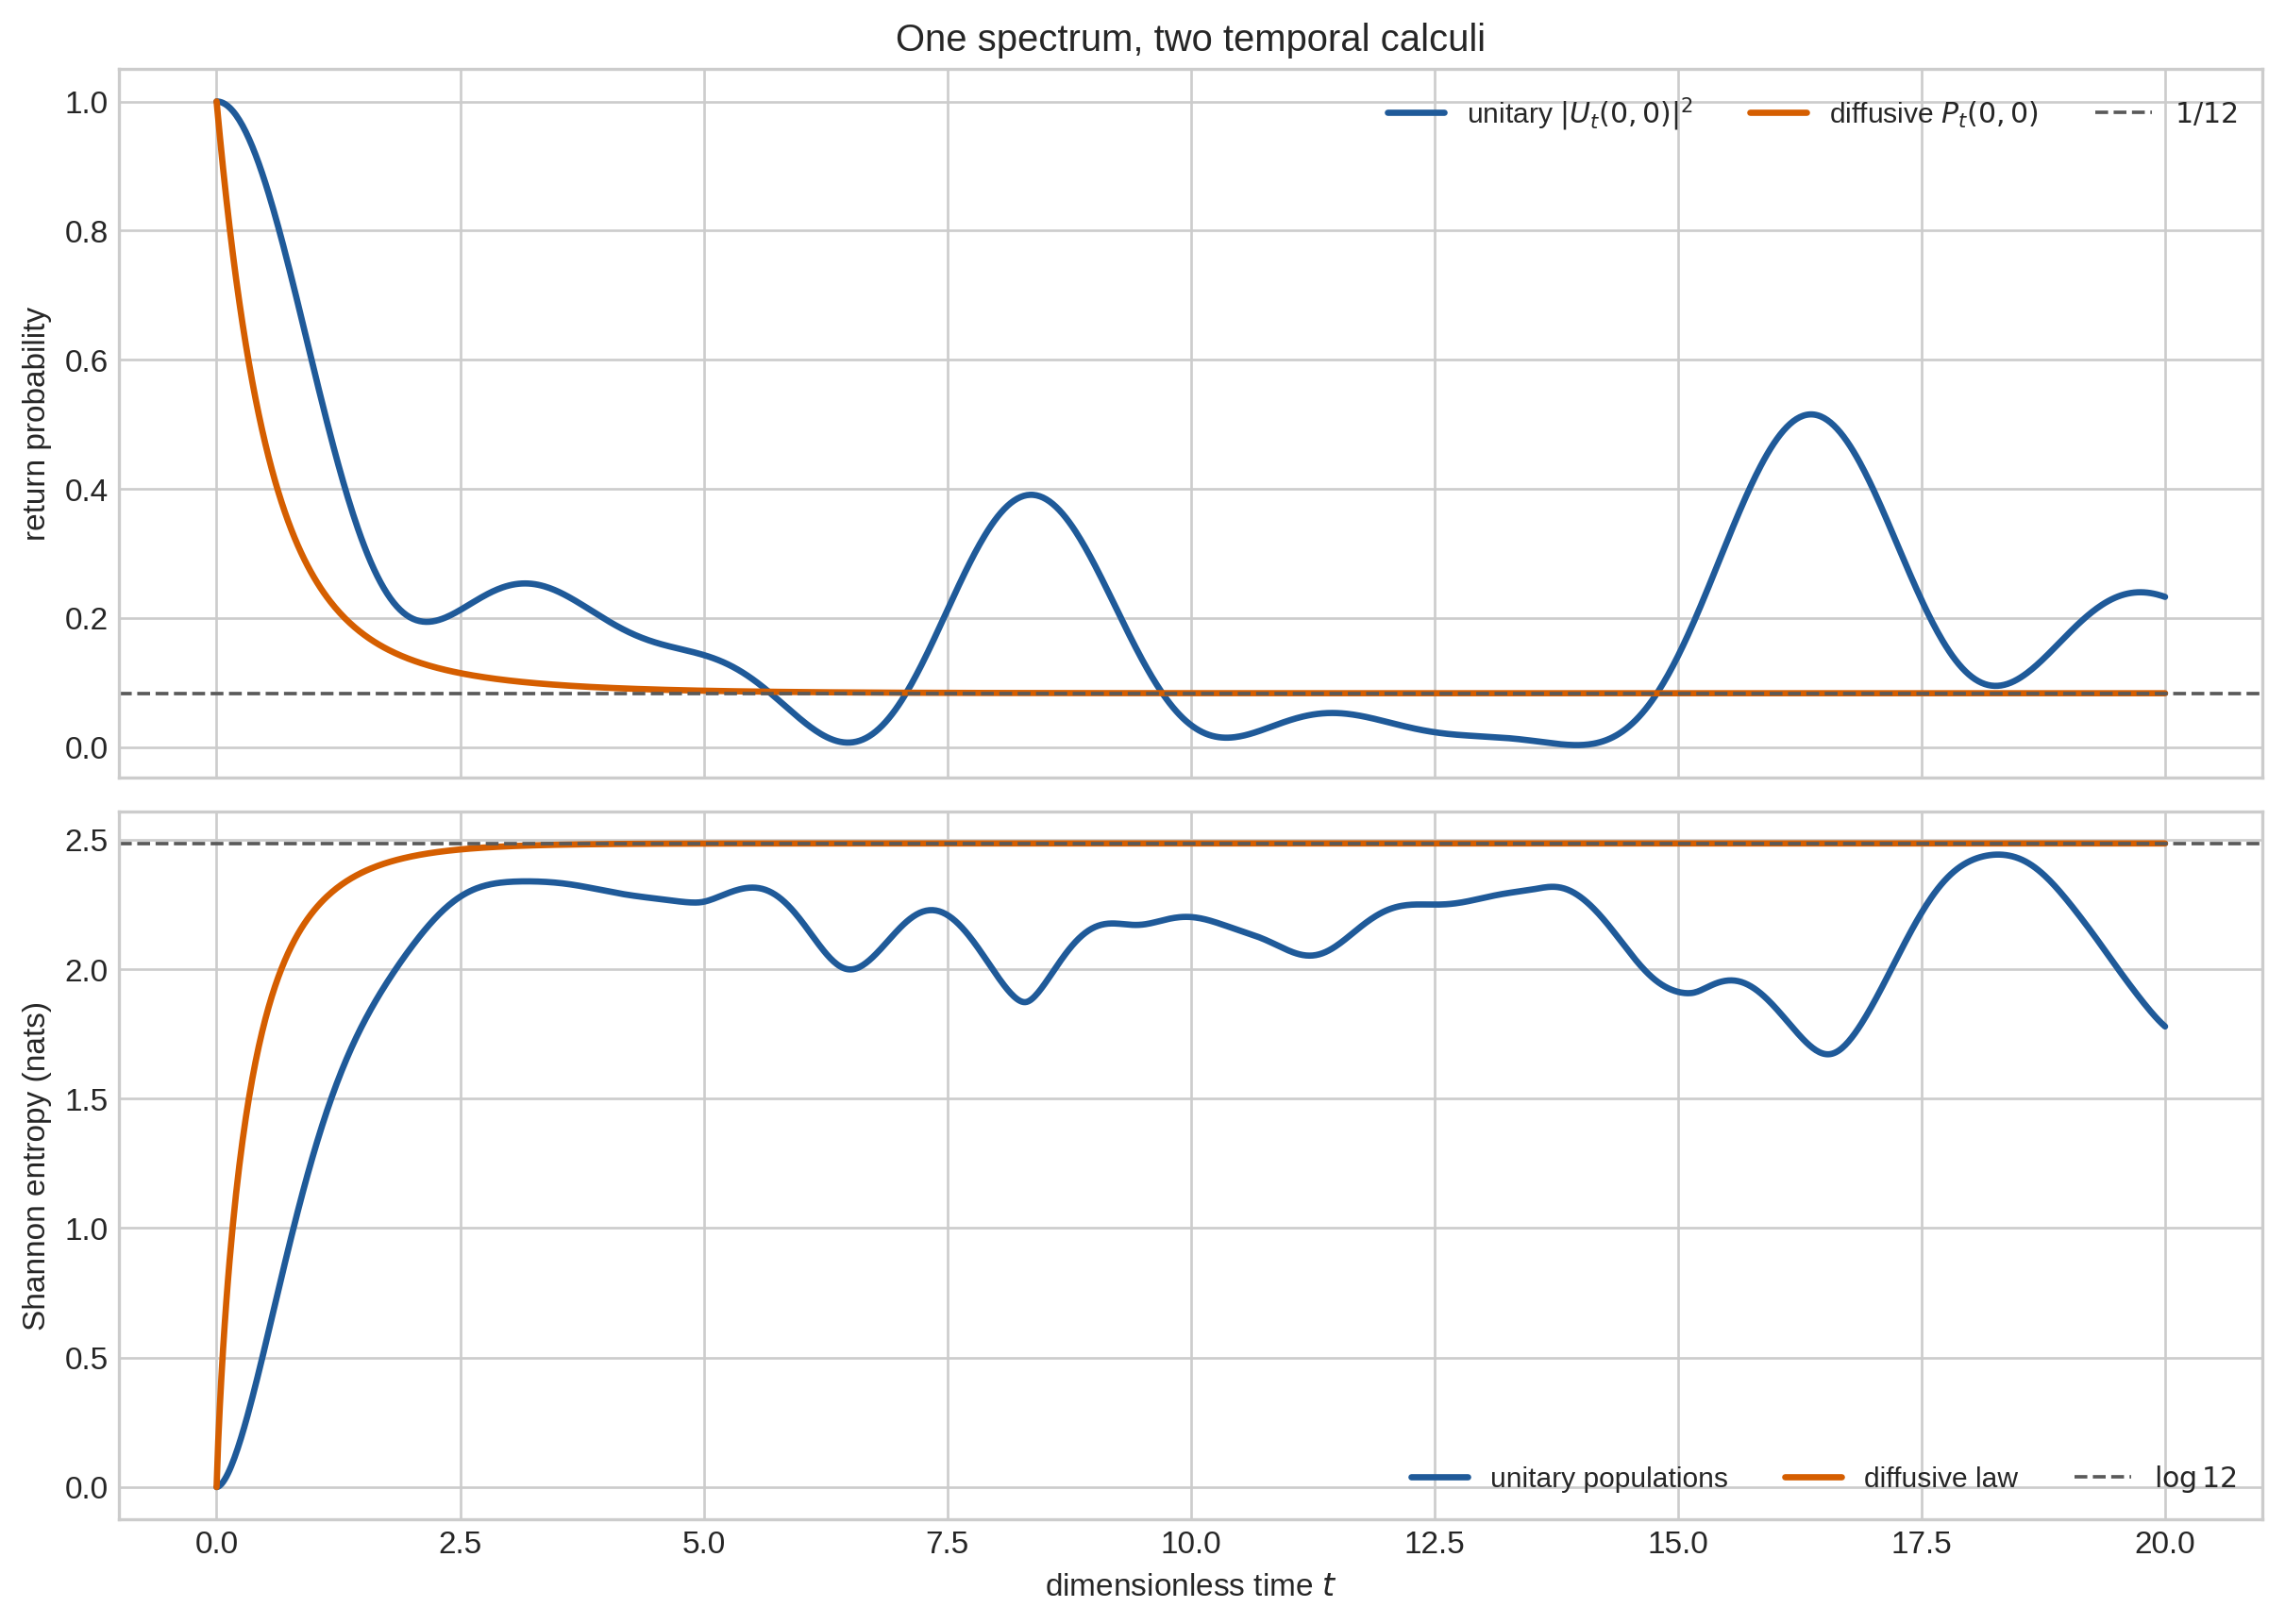
\includegraphics[width=0.94\textwidth]{FIN_One_Spectrum_Two_Dynamics.png}
\caption{\textbf{One spectrum, two temporal calculi.} Starting from a localized vertex, the Markov return probability converges to $1/12$ and its Shannon entropy to $\log12$. Unitary population entropy is nonmonotone because phase coherence is retained. Time is dimensionless; the plot does not supply a physical clock.}
\label{fig:two-calculi}
\end{figure}

\section{A finite double-slit operational experiment}

\subsection{Protocol}

This section implements the requested double-slit simulation in the smallest honest form supported by the matrix. It is a two-path interferometer with a twelve-outcome detector, not a finite-difference approximation to the free Schrödinger equation in Euclidean space.

Choose slit vertices
\[
 a=-2\equiv10\pmod{12},\qquad b=+2.
\]
A phase-controlled preparation with environmental record states is
\[
 |\Psi_{\phi}\rangle
 =\frac{|a\rangle|E_a\rangle+e^{i\phi}|b\rangle|E_b\rangle}{\sqrt2},
 \qquad \eta=\langle E_b|E_a\rangle.
\]
For the plotted cases $\eta\in[0,1]$ is real. The twelve detector effects are $D_x=|x\rangle\langle x|$. After unitary propagation, write
\[
 u_a(x,t)=\langle x|U_t|a\rangle,\qquad
 u_b(x,t)=\langle x|U_t|b\rangle.
\]
Tracing out the path record gives
\begin{equation}\label{eq:interference-law}
 p_{\phi,\eta}(x,t)
 =\frac{|u_a|^2+|u_b|^2}{2}
 +\Re\!\left(\eta e^{-i\phi}u_a\overline{u_b}\right).
\end{equation}
The three compared laws are:
\begin{enumerate}[label=(\roman*)]
\item coherent interference: $\eta=1$ and $\phi=0$;
\item an incoherent quantum mixture / perfectly distinguishing which-path record: $\eta=0$;
\item classical diffusion from $q_0=(\delta_a+\delta_b)/2$, namely $q_t=P_tq_0$.
\end{enumerate}

Equation~\eqref{eq:interference-law} is the operational bridge in miniature. $A$ supplies $U_t$, but the phase $\phi$, the coherence $\eta$, the slit preparation and the detector POVM are independent experimental data.

\subsection{Computed result}

Define the total interference magnitude
\[
 \mathcal I(t)=\frac12\sum_x|p_{0,1}(x,t)-p_{0,0}(x,t)|.
\]
The first local maximum on $0<t\le5$ occurs at
\[
 \boxed{t_*=1.5525},\qquad \boxed{\mathcal I(t_*)=0.1232806696}.
\]
These are grid-resolved floating-point values from the supplied reproducibility script. All three displayed probability vectors sum to $1$ within $2\times10^{-15}$.

At the symmetry detector $x=0$, reflection invariance gives $u_a=u_b$. Hence
\[
 p_{\phi,\eta}(0,t)=m_0(t)\,[1+\eta\cos\phi],
 \qquad m_0(t)=|u_a(0,t)|^2.
\]
At $t_*$,
\[
 m_0=0.07857926205,qquad
 p_{\max}=0.15715852410,qquad p_{\min}\approx0.
\]
The ideal visibility $(p_{\max}-p_{\min})/(p_{\max}+p_{\min})$ is therefore $1$. More generally the visibility at that detector is $|\eta|$: an orthogonal apparatus/environment record destroys the fringe, while erasing which-path distinguishability restores it.

\begin{figure}[H]
\centering
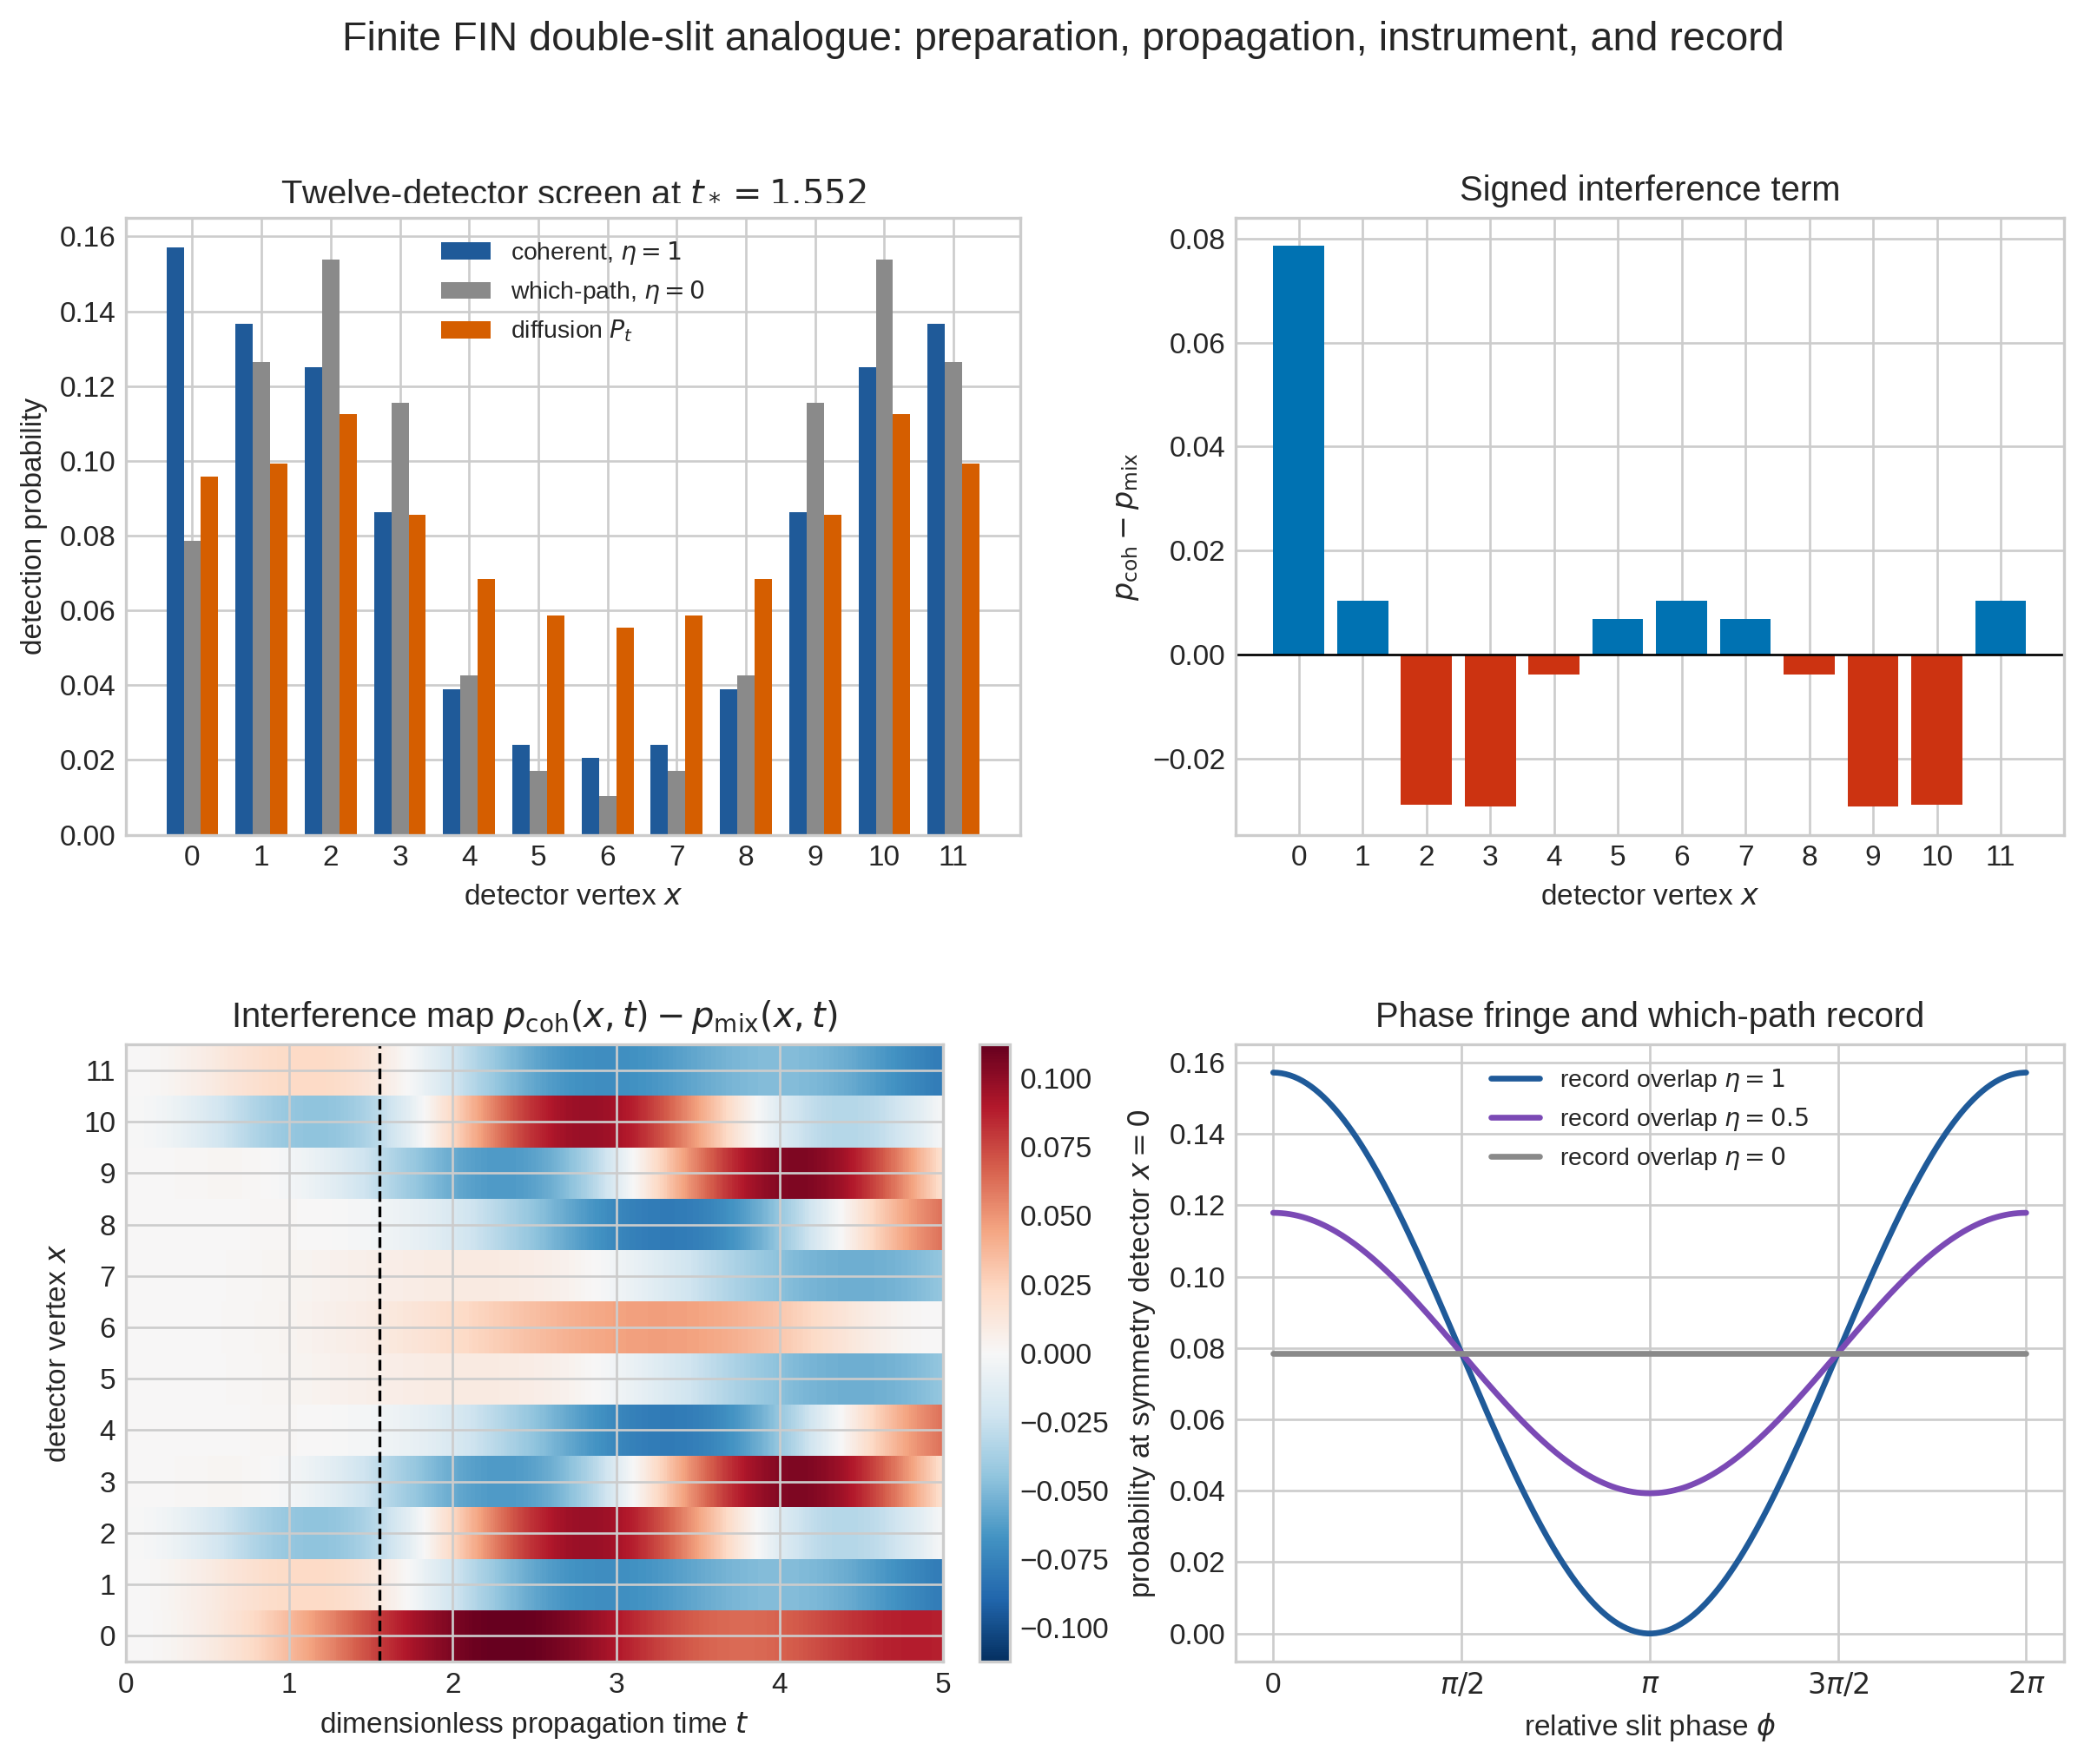
\includegraphics[width=\textwidth]{FIN_Double_Slit_Operational_Simulation.png}
\caption{\textbf{Finite double-slit analogue generated by $A$.} Top left: the coherent two-slit preparation, the dephased/which-path mixture and classical diffusion at the first interference maximum. Top right: the signed cross term, whose total sum is zero but whose detector-resolved pattern is nonzero. Bottom left: its evolution over all twelve detector outcomes. Bottom right: phase scanning at the symmetry detector; reducing the environment-record overlap $\eta$ removes the fringe. This figure simulates an explicitly specified operational protocol on $\Z_{12}$, not continuum diffraction.}
\label{fig:double-slit}
\end{figure}

\subsection{Why an intermediate observation changes composition}

Without an intermediate measurement, the amplitude is propagated by $U_{t+u}=U_tU_u$ before squaring. With a projective position measurement at time $u$, the phases are discarded and the observed population law composes as $B_tB_u$. The numerical Frobenius residual
\[
 \|B_{2t}-B_t^2\|_F
\]
is $0.04259$ at $t=0.1$, $0.72319$ at $t=0.5$, and $0.70674$ at $t=1$. By contrast $\|P_{2t}-P_t^2\|_F$ is analytically zero and appears near $10^{-15}$ numerically. The distinction is an instrument effect, exactly the ingredient absent from a bare operator-only description.

\section{Further numerical falsification tests}

\begin{table}[H]
\centering
\caption{One-site spreading from $\delta_0$. Entropies use natural logarithms and are in nats.}
\begin{tabular}{@{}ccccc@{}}
\toprule
$t$ & $|U_t(0,0)|^2$ & $H(|U_t\delta_0|^2)$ & $P_t(0,0)$ & $H(P_t\delta_0)$\\
\midrule
$0.1$ & $0.994634304$ & $0.040332484$ & $0.849358649$ & $0.716152665$\\
$1$   & $0.584353325$ & $1.293107954$ & $0.262829405$ & $2.225996234$\\
$5$   & $0.142549097$ & $2.259728107$ & $0.087250077$ & $2.484375810$\\
\bottomrule
\end{tabular}
\end{table}

\subsection{Mixing versus coherent memory}

For a localized Markov initial condition, the exact numerical total-variation mixing times are
\[
 t_{0.1}=2.4478902,\quad t_{0.05}=3.3576593,\quad
 t_{0.01}=5.4804113,\quad t_{0.001}=8.5307025.
\]
The unitary position law has no pointwise equilibrium. Its infinite-time Cesàro mean is
\[
 \overline p=(11/72,5/72,5/72,5/72,5/72,5/72,
 11/72,5/72,5/72,5/72,5/72,5/72),
\]
whose total-variation distance from uniform is $5/36\approx0.138889$. The enhancement at vertices $0$ and $6$ comes from the Fourier degeneracies. Thus even time averaging does not reproduce the Markov equilibrium.

\subsection{Why the Perron/Laplacian shift is essential}

The raw $W$ has negative eigenvalues. At $t=1$, $e^{-W}$ has row sum $0.19008056$, minimum entry $-0.43012412$ and operator norm $1.97758175$. It is neither stochastic nor contractive. In the unitary model the shift $sI$ changes only global phase; in the diffusive model it is the unique scalar correction that creates conservation. Treating the two shifts as physically interchangeable is therefore false.

\subsection{Failure of naive refinement}

The fixed analytic profile remains positive at $d=7$,
\[
 K(7)=0.0031528355,
\]
but becomes negative at $d=8$,
\[
 K(8)=-0.0017958784.
\]
A cyclic model first contains distance $8$ at $N=16$. Its off-diagonal Markov generator would then have a negative ``rate,'' and
\[
 (e^{tQ_N})_{xy}=t(Q_N)_{xy}+O(t^2)<0
\]
for sufficiently small $t$ at that separation. The Markov theorem is therefore certified at $N=12$ but does not survive naive fixed-parameter refinement. Truncation, rectification, absolute values or parameter running would each be a new axiom.

\section{The missing operational object}

The user-supplied diagnosis is substantially correct: a physical theory needs a structure that jointly specifies state, dynamics, clock, preparation, instrument, environment, apparatus and measurement record. A bare Hamiltonian or Markov generator specifies none of these as a complete experiment.

\subsection{Smallest standard completion}

\begin{definition}[Calibrated process--tester model]\label{def:cptm}
A calibrated process--tester model (CPTM) over ordered intervention slots $0,\ldots,n$ is the typed object
\[
 \mathfrak M=(\Upsilon_{n:0},\;\mathsf T,\;\mathsf C).
\]
Its components are:
\begin{enumerate}[label=(\alph*)]
\item a positive, causally normalized process tensor/quantum comb $\Upsilon_{n:0}$, which maps admissible interventions to multitime outcome probabilities;
\item a tester $\mathsf T=\{T_{\mathbf r|\mathbf a}\}$ made of completely positive instrument elements, including the first preparation slot and explicit classical outcome registers $\mathbf r$;
\item a clock/reference calibration $\mathsf C$ that associates physical clock readings and a reference frame with the ordered slots and their dimensionless parameters.
\end{enumerate}
The generalized Born rule is the link product, written schematically as
\[
 p(\mathbf r|\mathbf a,\mathsf C)
 =\Upsilon_{n:0}*T_{\mathbf r|\mathbf a},
\]
or, under a fixed Choi-transpose convention, as a trace pairing.
\end{definition}

This is one object in the sense of a typed operational model, not one unstructured matrix. Process tensors and quantum combs are established mathematics; the adjective ``calibrated'' records the extra clock/reference datum that these formalisms do not automatically generate.

\begin{theorem}[Role extraction, conditional on Definition~\ref{def:cptm}]
A CPTM determines all eight requested operational roles up to their natural operational equivalences:
\begin{center}
\begin{tabularx}{0.96\textwidth}{@{}>{\bfseries}lX@{}}
\toprule
Role & Carrier inside $\mathfrak M$\\
\midrule
State & Initial marginal / zero-slot restriction of $\Upsilon_{n:0}$\\
Dynamics & Conditional multitime maps and memory correlations in $\Upsilon_{n:0}$\\
Clock & Slot order, readings and dimensional calibration in $\mathsf C$\\
Preparation & First instrument element in $\mathsf T$\\
Instrument & Completely positive outcome-indexed maps in $\mathsf T$\\
Environment & Memory system in a minimal dilation of $\Upsilon_{n:0}$\\
Apparatus & A realization/dilation of the tester and reference frame\\
Record & Classical outcome register/pointer algebra indexed by $\mathbf r$\\
\bottomrule
\end{tabularx}
\end{center}
Minimal Stinespring realizations make environment and apparatus unique only up to isometry. A stronger claim of unique microscopic identity is neither operationally necessary nor mathematically available from the observed process alone.
\end{theorem}

\begin{proof}
The entries in the table are restrictions, marginals or dilations of the three typed components. Causal normalization makes probabilities consistent under omission of later instruments; complete positivity makes arbitrary ancillary extensions admissible; the tester supplies the interventions and records; calibration assigns operational time. Standard dilation theorems supply memory/environment and apparatus realizations, unique up to the appropriate isometries.
\end{proof}

\subsection{Necessity by deletion}

Each component is necessary for the requested coverage.

\begin{enumerate}
\item Remove $\Upsilon_{n:0}$: there is no law connecting interventions across time, no initial marginal and no environmental memory class.
\item Remove $\mathsf T$: there is no preparation, chosen instrument, apparatus realization or outcome record; $A$ alone gives no experimental probability.
\item Remove $\mathsf C$: one retains only an ordered, dimensionless family. Neither a physical duration nor an orientation/reference convention is fixed.
\end{enumerate}

Thus a bare process tensor is still insufficient for the user's full list, and a process plus instruments without calibration remains dimensionless. Conversely, no independent microscopic environment axiom is required for operational predictions because a dilation exists; specifying a particular microscopic bath is additional model detail.

\subsection{How $A$ enters, and where it stops}

$A$ can seed at least two inequivalent processes:
\[
 \mathcal U_t(\rho)=U_t\rho U_t^*,
\]
or the classical Markov process $P_t$ on the commutative position algebra. A Lindblad embedding with jump operators $L_{xy}=|x\rangle\langle y|$ and rates $W_{xy}$ can reproduce the Markov population equation, but that embedding also adds a choice of coherence dynamics. None is selected by $A$.

The double-slit calculation is a one-step CPTM instance: $U_t$ supplies the process, the two-slit channel supplies preparation, $|x\rangle\langle x|$ supplies the detector, $|E_a\rangle,|E_b\rangle$ supply an environment/apparatus record, and $t$ is the clock parameter. Changing any of these can change observed statistics without changing $A$.

\section{No-go results for deriving physics from $A$ alone}

\subsection{No absolute scale from dimensionless spectral data}

The displayed $A$ is dimensionless. Physical unitary and diffusive evolutions would require, respectively,
\[
 U_{\tau}^{\rm phys}=e^{-i(E_0/\hbar)\tau A},\qquad
 P_{\tau}^{\rm phys}=e^{-\kappa\tau A},
\]
with an energy $E_0$ or a rate $\kappa$.

\begin{proposition}[Scale obstruction]
No expression built solely from the entries of dimensionless $A$ by algebraic operations, limits and dimensionless spectral functional calculus can select a nonzero dimensional value of time, length, mass, energy or action.
\end{proposition}

\begin{proof}
All inputs and all operations are invariant under a change of physical unit. A proposed dimensional output would transform nontrivially under the scale group while its input is fixed, contradicting covariance. Equivalently, for every $c>0$, the pairs $(E_0,\tau)$ and $(cE_0,\tau/c)$ give identical dimensionless unitary predictions, and $(\kappa,\tau)$ and $(c\kappa,\tau/c)$ give identical Markov predictions. Nothing in $A$ selects one representative of either orbit.
\end{proof}

Clock calibration may \emph{supply} the missing scale; it cannot be claimed to derive it from $A$.

\subsection{No selector or orientation from the radial operator}

$W$ commutes with translations and reflections of $\Z_{12}$. Reflection exchanges modes $+m$ and $-m$ without changing their eigenvalues. Any selector choosing an absolute direction must therefore break a symmetry not broken by $A$. A chiral preparation or oriented apparatus can provide such a reference operationally, but this is an added resource, not strict-core selector closure.

\subsection{Information is not yet thermodynamic entropy}

$H(p)=-\sum_xp_x\log p_x$ in Figures~\ref{fig:two-calculi}--\ref{fig:double-slit} is dimensionless Shannon information in nats. Thermodynamic entropy requires a conversion scale such as $k_B$ and a physical ensemble; work or heat additionally requires temperature and a Hamiltonian/bath model. Landauer-type statements are conditional on those data. The CPTM supplies outcome statistics but does not turn $H$ into energy by itself.

\section{Shortest route to an experimental test}

A minimal test does not require cosmology or a continuum field theory.

\begin{enumerate}
\item Implement twelve controllable modes with a calibrated Hamiltonian $H=E_0A$ (photonic modes, trapped-ion modes or another programmable interferometer).
\item Prepare $(|10\rangle+e^{i\phi}|2\rangle)/\sqrt2$ and scan $\phi$.
\item Propagate for $\tau_*=1.5525\hbar/E_0$ and record the twelve-mode detector distribution.
\item Couple an ancilla to the path so that $\eta=\langle E_b|E_a\rangle$ can be tuned. Verify the predicted linear loss of visibility at detector $0$.
\item In a separate classical device, implement rates $Q_{xy}=W_{xy}$ for $x\ne y$ and $Q_{xx}=-s$. Compare its law at $\tau_*=1.5525/\kappa$ with the Markov curve, without identifying the two physical times unless $E_0/\hbar$ and $\kappa$ are independently calibrated.
\item Test multitime composition: the Markov transition matrices obey Chapman--Kolmogorov; coherent Born-position matrices do not unless an intermediate measurement is actually made.
\end{enumerate}

This would test the matrix implementation and the operational discrimination theorem. It would not establish that FIN uniquely governs nature: competing Hamiltonians or rate matrices must be included in statistical model comparison.

\section{Originality and comparison with existing mathematics}

\begin{table}[H]
\centering
\caption{What is standard and what is specific to this note.}
\begin{tabularx}{\textwidth}{@{}lXX@{}}
\toprule
Topic & Existing framework & Contribution here\\
\midrule
Dual functional calculus & Self-adjoint operators generate unitary groups; nonnegative graph Laplacians generate heat semigroups & Exact application, spectrum and boundary audit for the sampled FIN $12\times12$ matrix\\
Quantum walks & Continuous-time quantum walks and interference on finite graphs & FIN-weighted two-path predictions and reproducible figures\\
Classical diffusion & Reversible continuous-time Markov chains on weighted graphs & Exact rates, gap, mixing and refinement obstruction for this matrix\\
Instruments & Davies--Lewis instruments and POVMs & Identification of the missing preparation/instrument/record data in the FIN claim\\
Process tensors / combs & General multitime quantum processes with interventions and memory & Calibrated process--tester synthesis covering the eight requested roles\\
Relational clocks & Operational time from clock correlations/reference systems & Explicit proof that a clock calibration remains extra data\\
\bottomrule
\end{tabularx}
\end{table}

No novelty is claimed for the spectral theorem, graph-Laplacian positivity, quantum interference, Stinespring dilation or process-tensor formalism. The potentially useful contribution is the exact FIN-specific synthesis: it isolates what the operator proves, supplies a falsifiable finite experiment, and locates the irreducible operational and dimensional inputs.

\section{Confidence ledger and final answer}

\begin{longtable}{@{}p{0.22\textwidth}p{0.70\textwidth}@{}}
\toprule
Status & Statement\\
\midrule
\endhead
\proven & $A=sI-W$ is a connected weighted graph Laplacian on the stated $12$-vertex cyclic-distance convention.\\
\proven & $U_t$ is unitary and $P_t$ is an irreducible uniform-reversible Markov semigroup with shared Fourier projectors.\\
\proven & Born-position matrices from $U_t$ are not a nontrivial Markov semigroup; coherent and intermediate-measurement protocols differ.\\
\proven & The double-slit formula~\eqref{eq:interference-law} and ideal symmetry-detector visibility follow from the stated protocol.\\
\computed & The spectra, mixing times, Chapman--Kolmogorov residuals, $t_*$ and plotted distributions reproduce to the precision stated in the accompanying JSON file.\\
\proven & A dimensionful clock/rate cannot be generated from dimensionless $A$ without a dimensional calibration or equivalent scale resource.\\
\candidate & A calibrated process--tester model is the smallest established-style object found that jointly carries all eight requested operational roles.\\
\notestablished & $A$ uniquely selects unitary rather than diffusive physical time, a laboratory apparatus, an environment, a Born rule, an orientation, or dimensional constants.\\
\notestablished & The $N=12$ Markov result has a naive continuum/refinement limit; the fixed profile already violates nonnegative rates at distance $8$.\\
\bottomrule
\end{longtable}

The deepest defensible interpretation is therefore not that an observer chooses between wave and diffusion. It is that $A$ is a common spectral generator whose physical semantics are underdetermined until embedded in a calibrated process--tester model. The missing bridge is operational structure plus dimensional calibration. No theorem of the bare spectral operator can replace those inputs.

\section*{Reproducibility}

Run
\begin{verbatim}
python3 fin_dual_dynamics_release.py
\end{verbatim}
with Python 3, NumPy and Matplotlib. This regenerates
\path{FIN_Dual_Dynamics_reference_results.json},
\path{FIN_One_Spectrum_Two_Dynamics.png}, and
\path{FIN_Double_Slit_Operational_Simulation.png}.
The JSON records all displayed kernel weights, spectral values, numerical residuals and double-slit diagnostics. Floating-point residuals near $10^{-15}$ are not physical effects.

\begin{thebibliography}{99}

\bibitem{Chung}
F. R. K. Chung, \emph{Spectral Graph Theory}, CBMS Regional Conference Series in Mathematics 92, American Mathematical Society (1997).

\bibitem{FarhiGutmann}
E. Farhi and S. Gutmann, ``Quantum computation and decision trees,'' \emph{Physical Review A} \textbf{58}, 915--928 (1998). \href{https://doi.org/10.1103/PhysRevA.58.915}{doi:10.1103/PhysRevA.58.915}.

\bibitem{DaviesLewis}
E. B. Davies and J. T. Lewis, ``An operational approach to quantum probability,'' \emph{Communications in Mathematical Physics} \textbf{17}, 239--260 (1970). \href{https://doi.org/10.1007/BF01647093}{doi:10.1007/BF01647093}.

\bibitem{Stinespring}
W. F. Stinespring, ``Positive functions on $C^*$-algebras,'' \emph{Proceedings of the American Mathematical Society} \textbf{6}, 211--216 (1955). \href{https://doi.org/10.1090/S0002-9939-1955-0069403-4}{doi:10.1090/S0002-9939-1955-0069403-4}.

\bibitem{GKS}
V. Gorini, A. Kossakowski and E. C. G. Sudarshan, ``Completely positive dynamical semigroups of $N$-level systems,'' \emph{Journal of Mathematical Physics} \textbf{17}, 821--825 (1976). \href{https://doi.org/10.1063/1.522979}{doi:10.1063/1.522979}.

\bibitem{Lindblad}
G. Lindblad, ``On the generators of quantum dynamical semigroups,'' \emph{Communications in Mathematical Physics} \textbf{48}, 119--130 (1976). \href{https://doi.org/10.1007/BF01608499}{doi:10.1007/BF01608499}.

\bibitem{Supermaps}
G. Chiribella, G. M. D'Ariano and P. Perinotti, ``Transforming quantum operations: quantum supermaps,'' \emph{Europhysics Letters} \textbf{83}, 30004 (2008). \href{https://doi.org/10.1209/0295-5075/83/30004}{doi:10.1209/0295-5075/83/30004}.

\bibitem{Combs}
G. Chiribella, G. M. D'Ariano and P. Perinotti, ``Theoretical framework for quantum networks,'' \emph{Physical Review A} \textbf{80}, 022339 (2009). \href{https://doi.org/10.1103/PhysRevA.80.022339}{doi:10.1103/PhysRevA.80.022339}.

\bibitem{PollockPRL}
F. A. Pollock, C. Rodriguez-Rosario, T. Frauenheim, M. Paternostro and K. Modi, ``Operational Markov condition for quantum processes,'' \emph{Physical Review Letters} \textbf{120}, 040405 (2018). \href{https://doi.org/10.1103/PhysRevLett.120.040405}{doi:10.1103/PhysRevLett.120.040405}.

\bibitem{PollockPRA}
F. A. Pollock et al., ``Non-Markovian quantum processes: complete framework and efficient characterization,'' \emph{Physical Review A} \textbf{97}, 012127 (2018). \href{https://doi.org/10.1103/PhysRevA.97.012127}{doi:10.1103/PhysRevA.97.012127}.

\bibitem{PageWootters}
D. N. Page and W. K. Wootters, ``Evolution without evolution: dynamics described by stationary observables,'' \emph{Physical Review D} \textbf{27}, 2885--2892 (1983). \href{https://doi.org/10.1103/PhysRevD.27.2885}{doi:10.1103/PhysRevD.27.2885}.

\bibitem{GourSpekkens}
G. Gour and R. W. Spekkens, ``The resource theory of quantum reference frames: manipulations and monotones,'' \emph{New Journal of Physics} \textbf{10}, 033023 (2008). \href{https://doi.org/10.1088/1367-2630/10/3/033023}{doi:10.1088/1367-2630/10/3/033023}.

\bibitem{Shannon}
C. E. Shannon, ``A mathematical theory of communication,'' \emph{Bell System Technical Journal} \textbf{27}, 379--423 and 623--656 (1948). \href{https://doi.org/10.1002/j.1538-7305.1948.tb01338.x}{doi:10.1002/j.1538-7305.1948.tb01338.x}.

\bibitem{FINrepo}
K. Żuchowski, \emph{Fractal-Nadsoliton-Theory repository}, including the QW2118 finite-kernel data and subsequent mathematical reports, accessed 19 July 2026. \url{https://github.com/hyconiek/Fractal-Nadsoliton-Theory}.

\end{thebibliography}

\end{document}
